\documentclass[a4paper,titlepage]{article}

\usepackage[a4paper,left=20mm,right=20mm,top=15mm,bottom=2cm,includeheadfoot]{geometry}
\usepackage{ucs}
\usepackage[utf8x]{inputenc}
\usepackage[ngerman]{babel}
\usepackage{graphicx}
\usepackage{wrapfig}
\usepackage[colorlinks=true,linkcolor=black,citecolor=black,urlcolor=black]{hyperref}
\usepackage{listings}

% Palatino font
\usepackage[T1]{fontenc}
\usepackage[sc]{mathpazo}
\linespread{1.05}         % Palatino needs more leading (space between lines)

% section numbering
%\setcounter{secnumdepth}{-1}
%\setcounter{tocdepth}{1}

% section spacing
\setlength{\parskip}{0.2cm}
\setlength{\parindent}{0cm}

% fancy headers
\usepackage{fancyhdr}
\pagestyle{fancyplain}
%\renewcommand{\headrulewidth}{0pt}
\fancyhead{}
\fancyhead[L]{Dijkstra Spezifikation}
\fancyhead[R]{\footnotesize \thepage}
\fancyfoot{}

\title{Dijkstra Spezifikation\\Projektkette Naturwissenschaften}
\author{Adrian Boldi \and Igor Wiedler}

\begin{document}

\maketitle

\tableofcontents

\newpage

\section{Algorithmus}

\subsection{Problem}

Das Ziel des Dijkstra Algorithmus ist es, den kürzesten Weg zwischen zwei Punkten innerhalb eines gewichteten Graphes zu finden.

Ein mögliches Szenario hierfür ist eine Reise zwischen zwei Städten A und B. Zwischen diesen Städten befinden sich weitere Städte, welche durch Hauptstrassen verbunden sind. Das befahren dieser Hauptstrassen dauert unterschiedlich lange, was jedoch nicht nur von der eigentlichen Distanz abhängen muss. Das Ziel ist es den schnellsten weg zwischen A und B zu finden.

\subsection{Definition}

\begin{enumerate}
\item Dem Startknoten wird der Wert 0 zugewiesen. Dieser Knoten wird eingerahmt.
\item All jene Knoten, die mit dem zuletzt eingerahmten Knoten verbunden sind, werden mit dem Wert des gerahmten Knoten plus dem Wert der verbindenden Kante temporär beschriftet. Ist der Knoten bereits beschriftet, wird er nur dann überschrieben, wenn der neue Wert tiefer wäre als der bestehende. Bereits eingerahmte Knoten können hierbei ignoriert werden.
\item Von allen temporär beschrifteten, noch nicht eingerahmten Knoten wird derjenige eingerahmt, welcher den tiefsten Wert besitzt. Falls dieser Knoten der Zielknoten ist, gehe zu 5.
\item Gehe zurück zu 2.
\item Der schnellste Weg wurde gefunden.
\end{enumerate}

\subsection{Beispiel}

Hier soll der Algorithmus an einem einfachen Graphen gezeigt werden. Der Startknoten ist a, der Endknoten lautet f.

\begin{wrapfigure}{l}{0.48\textwidth}
\vspace{-5pt}
\begin{center}
	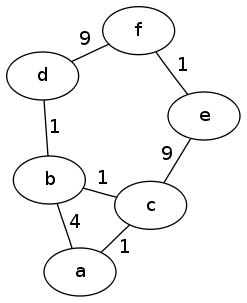
\includegraphics[width=4cm]{example.png}
\end{center}
\caption{Einfacher gewichteter Graph}
\vspace{-60pt}
\end{wrapfigure}

Knoten den Wert 0 zuweisen und einrahmen. \\ Verbundene Knoten beschriften: \emph{b = 4, c = 1}.

Tiefsten temporär beschrifteten Knoten einrahmen: \emph{c}. \\ Verbundene Knoten beschriften: \emph{b = 2, e = 10}.

Tiefsten temporär beschrifteten Knoten einrahmen: \emph{b}. \\ Verbundene Knoten beschriften: \emph{d = 3}.

Tiefsten temporär beschrifteten Knoten einrahmen: \emph{d}. \\ Verbundene Knoten beschriften: \emph{f = 12}.

Tiefsten temporär beschrifteten Knoten einrahmen: \emph{e}. \\ Verbundene Knoten beschriften: \emph{f = 11}.

Tiefsten temporär beschrifteten Knoten einrahmen: \emph{f}.

Der schnellste Weg lautet: \emph{f, e, c, a}.

\vspace{10pt}

Wie man leicht erkennen kann, wird der schnellste Weg gefunden, indem der Pfad welcher zum Einrahmen der jeweiligen Knoten geführt hat, rückwärts durchquert wird. Bei bedarf lässt sich dieser spiegeln, damit er beim Anfangsknoten beginnt und beim Zielknoten endet.

\section{Design}

\subsection{Programmablauf}

\begin{wrapfigure}{lh!}{0.5\textwidth}
\begin{center}
	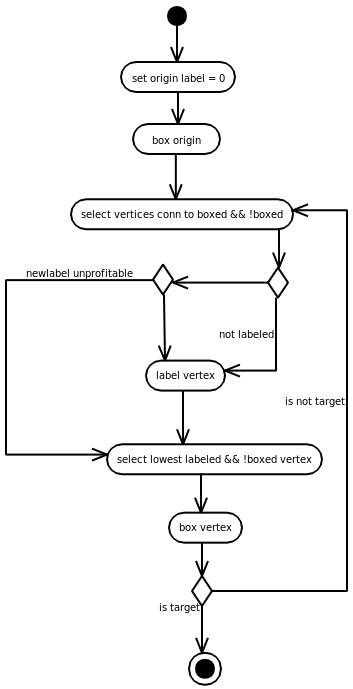
\includegraphics[width=7cm]{activity_diagram.png}
\end{center}
\caption{UML Aktivitätsdiagramm des Dijkstra}
\vspace{-60pt}
\end{wrapfigure}

Dieses Diagramm beschreibt den Ablauf des Dijkstra Algorithmus. Es entspricht der obrigen Definition.

\subsubsection*{Begriffe}

\begin{description}
\item[vertex] Knoten
\item[label] temporäre Beschriftung eines Knotens
\item[origin] Ursprung; der Ursprungsknoten des Algorithmus
\item[target] Ziel; der Zielknoten des Algorithmus
\item[boxed] permanent eingerahmt
\item[unprofitable] Vertex ist bereits temporär beschriftet, neuer Wert wäre jedoch höher oder gleich dem bestehenden
\item[lowest] der/die/das tiefste
\end{description}

\clearpage

\subsection{Datenmodell}

Es folgt ein Diagramm, welche die verwendeten Klassen, sowie deren Attribute und Beziehungen untereinander beschreibt. Diese Klassen definieren, welche Daten verwendet werden.

\begin{figure}[ht]
\begin{center}
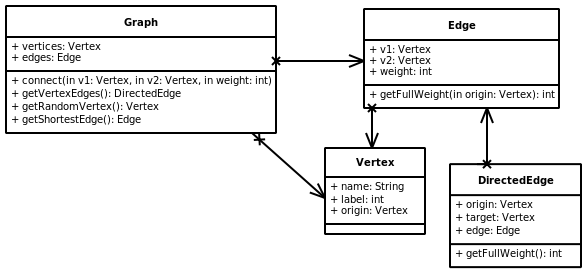
\includegraphics[width=0.7\textwidth]{model_diagram2.png}
\end{center}
\caption{UML Klassendiagramm des Modells}
\end{figure}

\subsubsection*{Beschreibung}

\begin{description}
\item[Graph] ein Graph beinhaltet Knoten und Kanten
\item[Vertex] ein Knoten
\item[Edge] eine gewichtete Kante zwischen zwei Knoten
\item[DirectedEdge] eine Kante, bei der die Richtung bekannt ist
\end{description}

\subsection{Anwendungsfälle}

Anwendungsfälle beschreiben die Funktionalitäten, die das Programm dem Benutzer bietet.

\begin{figure}[ht]
\begin{center}
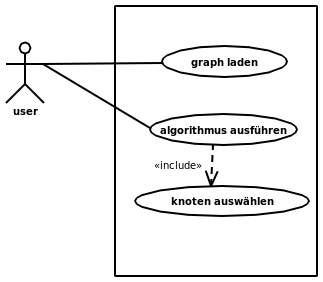
\includegraphics[width=0.4\textwidth]{usecases.png}
\end{center}
\caption{UML Anwendungsfall Diagramm}
\end{figure}

\subsubsection*{Beschreibung}

\begin{description}
\item[User] der Benutzer des Programms
\item[Graph laden] Graphen können aus einer Datei geladen werden
\item[Algorithmus ausführen] dies ist die Hauptfunktion
\item[Knoten auswählen] bei manchen Algorithmen (zum Beispiel Dijkstra) wird ein Start- und/oder Zielknoten benötigt, dieser soll ausgewählt werden können
\end{description}

\newpage

\section{Dateiformat}

\subsection{Allgemein}

Damit es möglich ist Graphen in das Programm zu laden, braucht es ein Dateiformat. Der Einfachheit halber wird hier ein ASCII basiertes Format verwendet. Eine Zeile in der Datei kann hierbei entweder einen Knoten oder eine Kante beschreiben.

Die Zeilen werden mittels Linefeed (\emph{ASCII 10}) getrennt. Pro Zeile gibt es Tokens, die via Tab (\emph{ASCII 9}) getrennt werden. Dies gleicht einem CSV-Format mit Tab Delimiter.

\begin{figure}[hb]
	\centering
	[typ] \hspace*{3em} \fbox{tab} \hspace{2.7em} [token] \hspace{3.4em} \fbox{tab} \hspace{2.7em} [token\_n] \hspace{3.7em} \fbox{linefeed}
	\caption{Grundgerüst des Dateiformats}
\end{figure}

\subsection{Typen}

Ein \emph{v} als Typ steht für einen Knoten (\emph{Vertex}), ein \emph{e} für eine Kante (\emph{Edge}). Je nach Typ gibt es verschiedene Tokens.

\vspace*{14pt}

\begin{minipage}{0.5\textwidth}
	\subsubsection{Vertex}

	\begin{description}
	\item[Name] Der Name des Knotens
	\item[Position x] Die x-Koordinate
	\item[Position y] Die y-Koordinate
	\end{description}
\end{minipage}
\begin{minipage}{0.5\textwidth}
	\subsubsection{Edge}

	\begin{description}
	\item[Von] Der Name des Ursprungsknotens
	\item[Nach] Der Name des Zielknotens
	\item[Gewichtung] Die Gewichtung der Kante
	\end{description}
\end{minipage}

\subsection{Beispiel}

\begin{figure}[h!]
\begin{center}
\begin{tabular}{| l r r r |}
\hline
\emph{v} & a & 5 & 5 \\
\emph{v} & b & 5 & 10 \\
\emph{v} & c & 10 & 5 \\
\emph{e} & a & b & 3 \\
\emph{e} & b & c & 4 \\
\hline
\end{tabular}
\end{center}
\caption{Beispiel eines einfachen Grafs}
\end{figure}

\subsection{Dateiendung}

Der einfachheit halber wird keine Dateiendung benötigt. Aus Kompatibilitätsgründen (Windows) ist es jedoch möglich eine \emph{txt} Endung zu verwenden.

\newpage

\section{Pseudocode}

\begin{lstlisting}
// eingabe entgegennehmen
input: vertices, origin, target

// initialisation
boxed = []

// origin vorbereiten
origin.label = 0
boxedVertex = origin

// endlosschlaufe
while true
	boxed += boxedVertex

	if boxedVertex == target
		// ziel erreicht
		break

	foreach getVertexEdges(boxedVertex) as edge
		// ueberspringen falls boxed
		// ueberspringen falls unprofitabel (nicht ueberschreibbar)
		if !boxed.contains(edge.target) ||
			(edge.target.label && edge.fullweight >= edge.target.label)

			edge.target.label = edge.fullweight
			edge.target.origin = boxedVertex

			// vertices nach label aufsteigend sortieren
			// tiefsten selektieren
			vertices.sort()
			foreach vertices as vertex
				if !boxed.contains(vertex) && vertex.label
					boxedVertex = vertex
					break

// auswertung
result = []

vertex = target
result += vertex

while vertex != origin
	vertex = vertex.origin
	result += vertex

output: result
\end{lstlisting}

\newpage

\section{Programmdokumentation}

\subsection{Generell}

Die Applikation \emph{UltraGraph} wurde in Java realisiert. Java enthält erweiterte Objektorientierte Features sowie eine einheitliche grafische Oberfläche und gute Unterstützung für die gängigsten Betriebssysteme.

Abstraktion wurde eingesetzt, um die Komponenten so lose wie möglich zu koppeln. Beispielsweise ist das GUI nicht von einem bestimmten Algorithmus abhängig, es kann mehrere verwenden. Ausserdem wurden Teile des Model-View-Controller Patterns eingesetzt, welche die Logik von Daten und Darstellung trennen.

Da der Quellcode weitgehend mit Javadoc kommentiert wurde, ist eine Javadoc-Dokumentation vorhanden.

\subsection{Klassen}

\subsubsection{Reader}

Die Klasse Reader ist dazu da, um die gespeicherten Graphen aus einer Text Datei auszulesen, und den Graph zu erzeugen.

Ablaufbeschreibung der Funktion \emph{getGraph}:

\begin{enumerate}
\item Aufruf der Funktion mit dem Namen des Files als Parameter.
\item Einlesen der ersten Linie.
\item Die Linien werden nun gesplitet
\item Der erste Character der Linie wird überprüft
\begin{itemize}\item Wenn \emph{v}, dann einen neuen Vertex mit den drei folgenden Characters
\begin{itemize}\item Vertex wird zu Graph \emph{g} hinzugefügt.\end{itemize}\end{itemize}
\begin{itemize}\item Wenn \emph{e}, dann eine neue Edge mit den drei folgenden Characters
\begin{itemize}\item Im Graph \emph{g} werden zwei Vertex mit der Edge verbunden.\end{itemize}\end{itemize}
\item Gibt den Graph \emph{g} zurück
\end{enumerate}

\subsubsection{Writer}

Die Klasse Writer ist dazu da, um den Graph in eine Text Datei zu speichern.

Ablaufbeschreibung:

\begin{enumerate}
\item Aufruf der Funktion mit den Parametern: Graph \emph{g} und des gewünschten Filename
\item Das File wird erstellt
\item Solange Vertices im Graph \emph{g} vorhanden sind
\begin{itemize}\item Schreibe Identifikation, Name, X-Koordinate und Y-Koordinate in das File\end{itemize}
\item Solange Edges im Graph \emph{g} vorhanden sind
\begin{itemize}\item Schreibe Identifikation, Start Vertex, End Vertex und Gewichtung in das File\end{itemize}
\item File wird geschlossen
\end{enumerate}

\subsubsection{Dijkstra}

In der Klasse Dijekstra ist der eigentliche Algorithmus implementiert. Eine genauere Beschreibung des Algorithmus finden sie in Punkt 2.1.

\subsubsection{Graph}

\begin{itemize}
\item Methode add(Vertex... vertices)
\begin{itemize}\item fügt alle Vertices in den Vektror Vertices hinzu.\end{itemize}
\item Methode connect(Vertex v1, Vertex v2, int weight)
\begin{itemize}\item erzeugt Edges und fügt diesen dem Vektor Edge hinzu.\end{itemize}
\item Methode connect(Vertex v1, Vertex v2)
\begin{itemize}\item erzeugt Edges mit einem Defaultwert für weight und fügt diesen dem Vektor Edge hinzu.\end{itemize}
\item Methode getVertices()
\begin{itemize}\item gibt alle Vertices zurück\end{itemize}
\item Methode getEdges()
\begin{itemize}\item gibt alle Edges zurück\end{itemize}
\item Methode removeVertex(Vertex v)
\begin{itemize}\item löscht den Vertex v mit allen angeschlossenen Edges\end{itemize}
\item Methode removeEdge(Edge e)
\begin{itemize}\item löscht die Edge e\end{itemize}
\item Methode removeVertices(Vector<Vertex> vv)
\begin{itemize}\item löscht alle Vertices vv\end{itemize}
\item Methode getVertexEdges(Vertex v)
\begin{itemize}\item gibt alle mit v verbundenen Edges zurück\end{itemize}
\item Methode getVerticesEdges(Vertex v1, Vertex v2)
\begin{itemize}\item gibt alle mit v1 und v2 verbundenen Vertices zurück\end{itemize}
\end{itemize}

\subsubsection{Vertex}

Die Klasse Vertex ist das Model für die Vertices.

\subsubsection{Edge}

Die Klasse Vertex ist das Model für die Edges.

\subsubsection{GraphGUI}

Die Klasse GraphGUI enthält das graphische Oberfläche von UltraGraph.

\subsubsection{Point}

Representiert die Koordinaten der Vertices.

\subsubsection{EdgeEditWindow}

Das Fenster für die Editierung eines Edges.

\subsubsection{VertexFactory}

Erstellt Vertex mit einem Namen.

\subsubsection{VertexEditWindow}

Das Fenster für die Editierung eines Vertex mit X- und Y-Position.

\subsubsection{ItemSelectWindow}

Auswahlfenster zum auswählen des gewünschten Edges oder Vertices zum editieren.

\subsection{Anwendung}

Wenn Sie UltraGraph starten erscheint das Hauptfenster. Die leere Fläche bietet Platz für Ihren Graphen.

\begin{figure}[ht]
\begin{center}
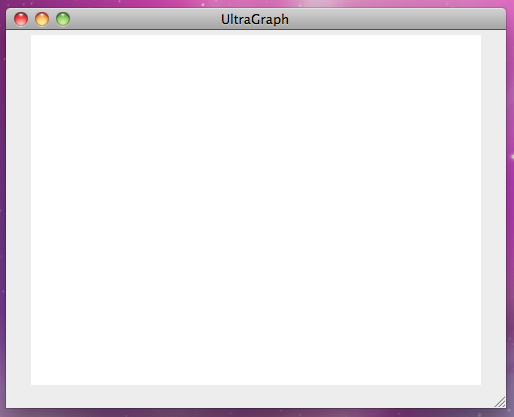
\includegraphics[width=0.7\textwidth]{screenshot/main_window.png}
\end{center}
\end{figure}

\subsubsection{Graphen}

Nach dem Programmstart erscheint ein neuer leerer Graph. Falls Sie den momentanen Graph verwerfen wollen, drücken Sie \emph{Command + N}, um einen neuen zu erzeugen. Über \emph{Graph $\rightarrow$ New} besteht eine alternative Möglichkeit hierfür.

Falls Sie einen gespeicherten Graphen laden wollen, drücken Sie \emph{Command + O}, und wählen Sie die Datei aus, welche den Graphen enthält. Über \emph{Graph $\rightarrow$ Open} besteht eine alternative Möglichkeit hierfür.

Um einen Graphen zu speichern, drücken Sie \emph{Command + S}. Ein Graph kann in verschiedenen Formaten gespeichert werden: Das UltraGraph-Format, Graphviz-dot und XStream-XML. Wählen Sie den Ort und den Dateinamen für die Datei. Über \emph{Graph $\rightarrow$ Save} besteht eine alternative Möglichkeit hierfür.

\subsubsection{Vertices}

Um einen Vertex hinzuzufügen, muss mit gedrückter Alt-Taste auf die Position geklickt werden, an welcher der neue Vertex erscheinen soll. Über \emph{Vertex $\rightarrow$ Add} besteht eine alternative Möglichkeit hierfür.

Vertices können verschoben werden, indem der Vertex mit gedrückter Maustaste an die gewünschte stelle gezogen wird. Über \emph{Vertex $\rightarrow$ Edit} besteht eine alternative Möglichkeit hierfür, bei der es auch möglich ist Vertices umzubenennen.

Um einen Vertex zu löschen, muss mit gedrückten Shift- und Alt-Tasten auf den Vertex geklickt werden, welcher gelöscht werden soll. Über \emph{Vertex $\rightarrow$ Remove} besteht eine alternative Möglichkeit hierfür.

\subsubsection{Edges}

Um eine Edge hinzuzufügen, müssen die beiden zu verbindenden Vertices mit gedrückter Shift-Taste verbunden werden. Die neue Edge erscheint dann. Es ist auch möglich mehrere Edges zwischen zwei Vertices zu haben. Über \emph{Edge $\rightarrow$ Add} besteht eine alternative Möglichkeit hierfür.

Die Gewichtung von Edges kann geändert werden, indem im Menü \emph{Vertex $\rightarrow$ Edit} ausgewählt wird.

Um eine Edge zu löschen, selektiert man im Menü \emph{Vertex $\rightarrow$ Remove}.

\subsubsection{Algorithmen}

UltraGraph beherscht sowohl den Dijkstra-Algorithmus, wie auch Kruskal und Prim. Um den zu verwendenden Algorithmus auszuwählen muss man \emph{Command + A} oder im Menü \emph{Algorithm $\rightarrow$ Select algorithm} wählen.

Um den ausgewählten Algorithmus zu starten, wird \emph{Command + R} gedrückt, oder im Menü \emph{Algorithm $\rightarrow$ Start} ausgewählt. Im Falle das Dijkstra, muss noch konfiguriert werden, welches die Start- und Endknoten sein sollen, bei den anderen beiden ist keine Konfiguration nötig. Sobald diese vorgenommen wurde, wird der Algorithmus gestartet. Die Anzeige erfolgt direkt im Hauptfenster.

Es ist möglich, den laufenden Algorithmus via \emph{Algorithm $\rightarrow$ Pause} zu pausieren.

Falls das Programm auf der Kommandozeile ausgeführt wird, werden dort zusätzliche Informationen angezeigt.

\newpage

\subsection{Beispiele}

\begin{figure}[h!]
\begin{center}
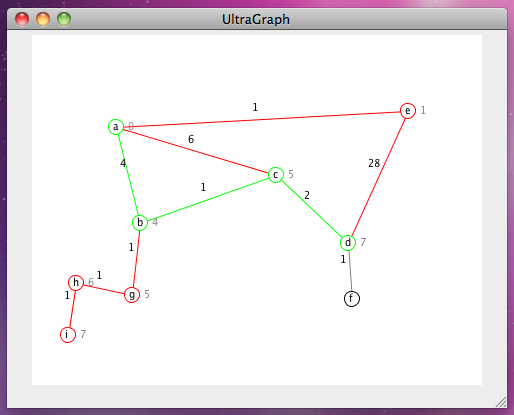
\includegraphics[width=0.7\textwidth]{screenshot/example.png}
\end{center}
\caption{Beispielsgraph nach Dijkstra Durchlauf}
\end{figure}

\begin{figure}[h!]
\begin{center}
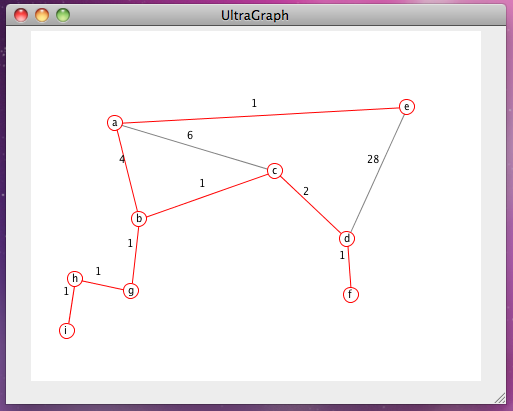
\includegraphics[width=0.7\textwidth]{screenshot/example2.png}
\end{center}
\caption{Beispielsgraph nach Kruskal Durchlauf}
\end{figure}

\newpage

\begin{figure}[h!]
\begin{center}
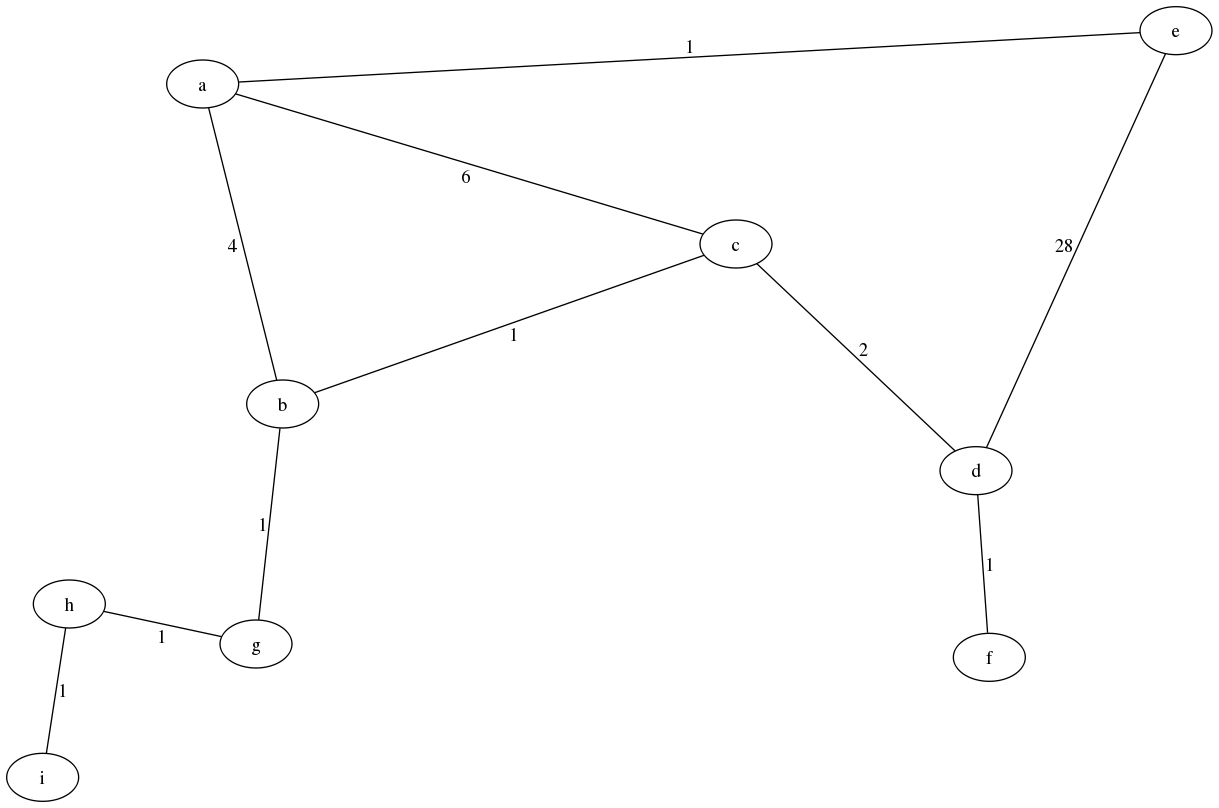
\includegraphics[width=\textwidth]{screenshot/example_dot.png}
\end{center}
\caption{Beispielsgraph mit Graphviz visualisiert}
\end{figure}

\newpage

\section{Verwendete Mittel}

\subsection{Programme}

\begin{itemize}
\item \emph{Eclipse:} Entwicklungsumgebung für Java \\
	\emph{\href{http://www.eclipse.org}{http://www.eclipse.org}}
\item \emph{Gaphor} UML Diagramm Tool \\
	\emph{\href{http://gaphor.sourceforge.net}{http://gaphor.sourceforge.net}}
\item \emph{Graphviz} Graphenvisualisierung \\
	\emph{\href{http://graphviz.org}{http://graphviz.org}}
\item \LaTeX: Textsatz-Software \\
	\emph{\href{http://www.latex-project.org}{http://www.latex-project.org}}
\item \emph{XStream}: Java XML-Enkodierungs-Bibliothek \\
	\emph{\href{http://xstream.codehaus.org}{http://xstream.codehaus.org}} \\
	\emph{\href{http://www.extreme.indiana.edu/xgws/xsoap/xpp/mxp1/index.html}{http://www.extreme.indiana.edu/xgws/xsoap/xpp/mxp1/index.html}}
\end{itemize}

\subsection{Quellen}

\subsubsection{WWW}

\begin{itemize}
\item vkaul: \emph{Dijkstra's Alhorithm}, 23. Januar 2004, 12. Januar, 2010 \\
	\emph{\href{http://ocw.mit.edu/NR/rdonlyres/Sloan-School-of-Management/15-082JNetwork-OptimizationSpring2003/FC13EFA1-0FE2-4BFB-B019-8939606EDDCC/0/dijkstrasalgorithm.pdf}{http://ocw.mit.edu/NR/rdonlyres/Sloan-School-of-Management/15-082JNetwork-OptimizationSpring2003/ \\
	FC13EFA1-0FE2-4BFB-B019-8939606EDDCC/0/dijkstrasalgorithm.pdf}}
\item Unbekannter Author: \emph{Der Algorithmus von Dijkstra}, 31. März 1998, 12. Januar, 2010 \\
	\emph{\href{http://www.educ.ethz.ch/lehrpersonen/informatik/unterrichtsmaterialien_inf/kommuniation_kryptographie/routing/la3.pdf}{http://www.educ.ethz.ch/lehrpersonen/informatik/unterrichtsmaterialien\_inf/kommuniation\_kryptographie/ \\
	routing/la3.pdf}}
\item Wikipedia: \emph{Algorithmus von Kruskal}, 18. August 2009, 12. Januar 2010 \\
	\emph{\href{http://de.wikipedia.org/wiki/Algorithmus_von_Kruskal}{http://de.wikipedia.org/wiki/Algorithmus\_von\_Kruskal}}
\item Jean-Philippe Rameau: \emph{Algorithmus von Kruskal Info}, unbekannte Datierung, 12. Dezember 2009 \\
	\emph{\href{http://infofrosch.info/a/al/algorithmus_von_kruskal.html}{http://infofrosch.info/a/al/algorithmus\_von\_kruskal.html}}
\item Papagelis Athanasios: \emph{Kruskal Algorithm}, 13. Oktober 1997, 12. Januar 2010 \\
	\emph{\href{http://students.ceid.upatras.gr/~papagel/project/kruskal.htm}{http://students.ceid.upatras.gr/$\sim$papagel/project/kruskal.htm}}
\item Papagelis Athanasios: \emph{Pseudocode For Kruskal Algorithm}, 13. Oktober 1997, 12. Januar 2010 \\
	\emph{\href{http://students.ceid.upatras.gr/~papagel/project/pseukrus.htm}{http://students.ceid.upatras.gr/$\sim$papagel/project/pseukrus.htm}}
\item Wikipedia: \emph{Algorithmus von Prim}, 13. September 2008, 12. Januar 2010 \\
	\emph{\href{http://de.wikipedia.org/wiki/Algorithmus_von_Prim}{http://de.wikipedia.org/wiki/Algorithmus\_von\_Prim}}
\item Kenji Ikeda, William F. Klostermeyer: \emph{Prim's Algorithm Demo}, 6. Juli 2001, 12. Januar 2010 \\
	\emph{\href{http://www.unf.edu/~wkloster/foundations/PrimApplet/PrimApplet.htm}{http://www.unf.edu/$\sim$wkloster/foundations/PrimApplet/PrimApplet.htm}}
\item Jean-Michel Léon: \emph{Implementing Double Buffering with Java}, 27. September 2006, 12. Januar 2010 \\
	\emph{\href{http://www.ecst.csuchico.edu/~amk/classes/csciOOP/double-buffering.html}{http://www.ecst.csuchico.edu/$\sim$amk/classes/csciOOP/double-buffering.html}}
\item Unbekannter Author: \emph{The DOT Language}, unbekannte Datierung, 12. Januar 2010 \\
	\emph{\href{http://www.graphviz.org/doc/info/lang.html}{http://www.graphviz.org/doc/info/lang.html}}
\end{itemize}

\subsubsection{Literatur}
\begin{itemize}
\item \emph{Networks -- Student text and unit guide}, Cambridge University Press, 2000
\end{itemize}

\end{document}
